%% IMPORTANT: Once working, run latex 3 times to get listoffigures to work

%% Be sure to check spelling!

%% Put your name and the proper due date in place

%% Copy the lstinputlisting and figure code as many times as you need
%% Be sure to put in your own file names if appropriate

%% Note that the \epsfig and \lstinputlisting commands 
%% are currently commented out with %%% - until the
%% files exist, processing this code without them will result in an error
%% so leave the comments until you have created the files!

\documentclass{article}
\usepackage{amsmath}    % loads AMS-Math package
\usepackage{epsfig}     % allows PostScript files
\usepackage{listings}   % allows lstlisting environment
\usepackage{moreverb}   % allows listinginput environment
\usepackage[letterpaper, margin=0.75in]{geometry}  % set paper size/margins
\usepackage{EGR103F19}  % colorful file imports

\begin{document}
\begin{center}
\rule{6.5in}{0.5mm}\\~\\
\textbf{\large EGR 103L -- Fall 2019}\\~\\
\textbf{\huge Lab 5: Structured Programming II}\\~\\
***Marcus Deans (md374)***\\
***Lab Section 2, Tuesdays 11:45 - 2:35 ***\\
***13 October 2019***\\~\\
{\small I understand and have adhered to all the tenets of the Duke
  Community Standard in completing every part of this assignment.  I
  understand that a violation of any part of the Standard on any part
  of this assignment can result in failure of this assignment, failure
  of this course, and/or suspension from Duke University.} 
\rule{6.5in}{0.5mm}\\
\end{center}
\tableofcontents
\listoffigures
\pagebreak

\section{P\&E 4.46}
%%% Uncomment this once you have the file
\lstinputlisting[basicstyle=\ttfamily]{Coded.txt}

\section{P\&E 4.49}
%%% Uncomment this once you have the file
\lstinputlisting[basicstyle=\ttfamily]{dcs_scramble.txt}

\section{Chapra 4.25}
The graphs for the cos series approximator were very interesting, particularly in comparing the graphs representing identical angles but at different positions along the
function. While these graphs would, in an ideal and properly coded program, be identical, the results were anything but. For the graphs $\pi/4$ and $1.02\pi/2$, the
approximation value ``balanced'' out after several terms to yield similar approximations with each successive term (achieved around the fourth term). By the time the
calculations were stopped as a result of the relative error reaching the specified limit, the approximations were near the limit of improving their own accuracy. The values
of the approximation themselves were highly similar to the actual value of the cosine value at that position. In sum, the approximation worked well for these two values.

Different results were achieved with the graphing of $9\pi/4$ and $41.02\pi/2$. For the graph of $9\pi/4$, the approximation initially was highly inaccurate and whiplashed
to further positive and negative values. The approximation actually increased in distance from the origin for the first three terms. After the third term, however, the approximation increased in accuracy to yield similar values to that of the identical value $\pi/4$. The approximation similarly ceased when the relative error reached the threshold; this was in fact only met with a greater number of terms (~22) compared to the preceding functions. The graph of $41.02\pi/2$ was perhaps the most interesting, the approximation actually increased in inaccuracy with each successive term and when the relative error threshold was met, the approximation was not accurate at all. It was also interesting to note that the number of terms required for the approximation to cease (by meeting the thresholds) increased with a greater input value (regardless of it being the same angle as a prior input value). The number of terms in each approximation increased from $\sim$9 to $\sim$12 to $\sim$22 and finally to $\sim$30. 

\section{Finding Roots}
I found the graphs of the roots to be interesting, particularly for a function that, at first glance,
appears to be quite simple. The Map to Find Roots graph clearly illustrates the relation between $x_k$ and $x_{k+1}$. 
It was very interesting to see the Root Estimate graph; unexpectedly, there were not three distinct domains in which the initial guesses
corresponded to the same actual root. These existed only for three sections of the domain; there were also four other points at which a certain initial guess
would yield a root that would also be identified using a different initial guess along the domain. Specifically, an initial guess between 0 and 1 would yield a root
of 1.0, and an initial guess of 3 would \textbf{also} yield a root of 1.0. However, a guess between 1 and 3 could yield either 1.0, 2.0 or 4.0 as the root. This was unexpected
based only on the code. I expected three separate segments that would comprise a piecewise function, with steps between each level. I was not expecting such a 
degree of variability and fluctuation in the obtained root over very similar initial guess values. 

The iteration count graph, while initially confusing, was much more comprehensible when related to the root estimate graph. Around the more complex initial guess values 
- those for which a greater number of possible actual roots could be obtained from x-values similar to that of the initial guess (~1.5, for example) - there was a marked
increase in the number of iterations necessary to yield the correct root result. There was also a logical connection between the initial guess being very similar to the
actual root value and the (lower) number of iterations necessary to yield that root, considering that the initial guess was relatively accurate.  

The images were very interesting to see, particularly as I did not know that the graphs could be visualized in such a way. They seem to more simply communicate the
result using a colour scheme, and they also effectively demonstrate the gradient of the results. The drawbacks appear to be in the lack of clarity when trying to find
a specific result using such an image.

\pagebreak
\appendix
\section{Codes}
% Put the name of your file in the subsection name 
% and the listinginput input
% Be sure to include the community standard in codes!
% Add \pagebreaks if they make sense

%%% Uncomment as needed

\lstset{style=python103, language=python} 

\subsection{swap\_letters.py}
\lstinputlisting{swap_letters.py}
\clearpage

\subsection{scrambler.py}
\lstinputlisting{scrambler.py}
\clearpage

\subsection{cos\_series.py}
\lstinputlisting{cos_series.py}
\clearpage

\subsection{poly\_root.py}
\lstinputlisting{poly_root.py}
\clearpage 

% start Figures on new page

\section{Figures}
\begin{figure}[ht!]
\begin{center}
\begin{tabular}{cc}
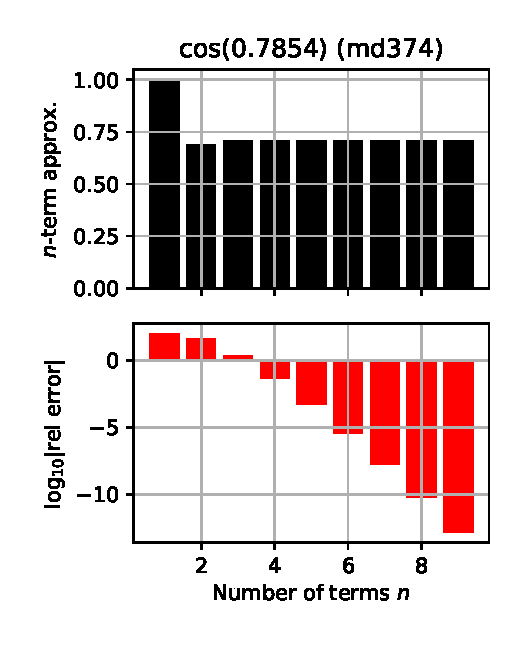
\epsfig{file=CosPlot0.eps} &
\epsfig{file=CosPlot1.eps} \\
\epsfig{file=CosPlot2.eps} &
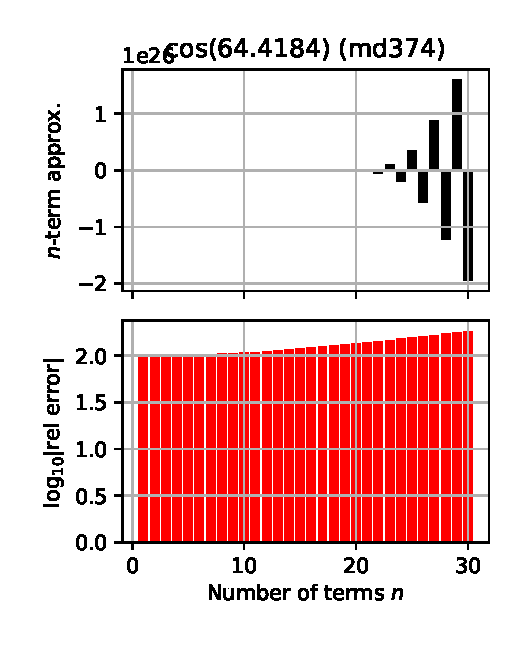
\epsfig{file=CosPlot3.eps} 
\end{tabular}
\caption{Figures for Cosine Approximation}
\end{center}
\end{figure}
\clearpage
\begin{figure}[ht!]
\begin{center}
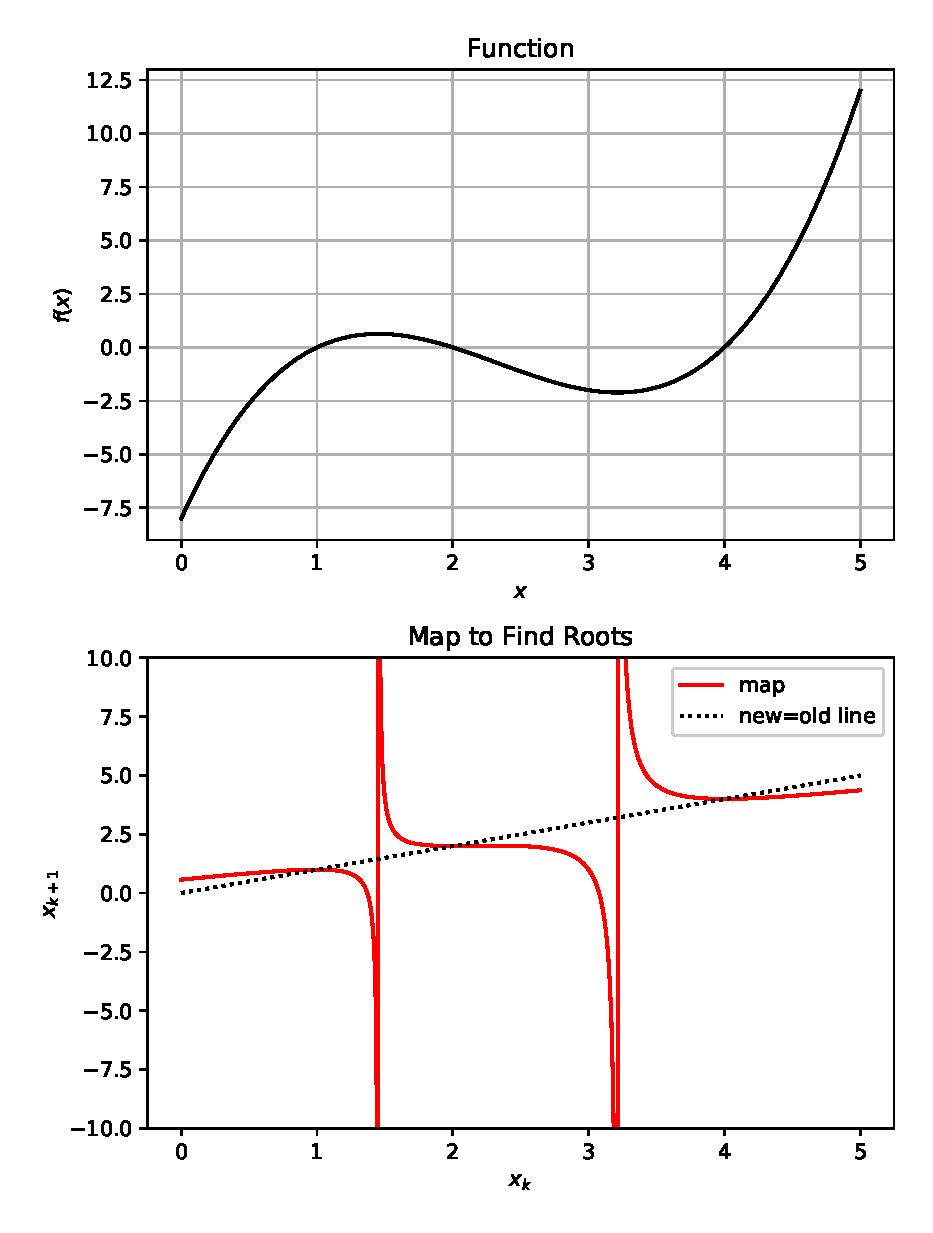
\epsfig{file=RootPlot0.eps} 
\caption{Function and Derivative}
\end{center}
\end{figure}
\begin{figure}[ht!]
\begin{center}
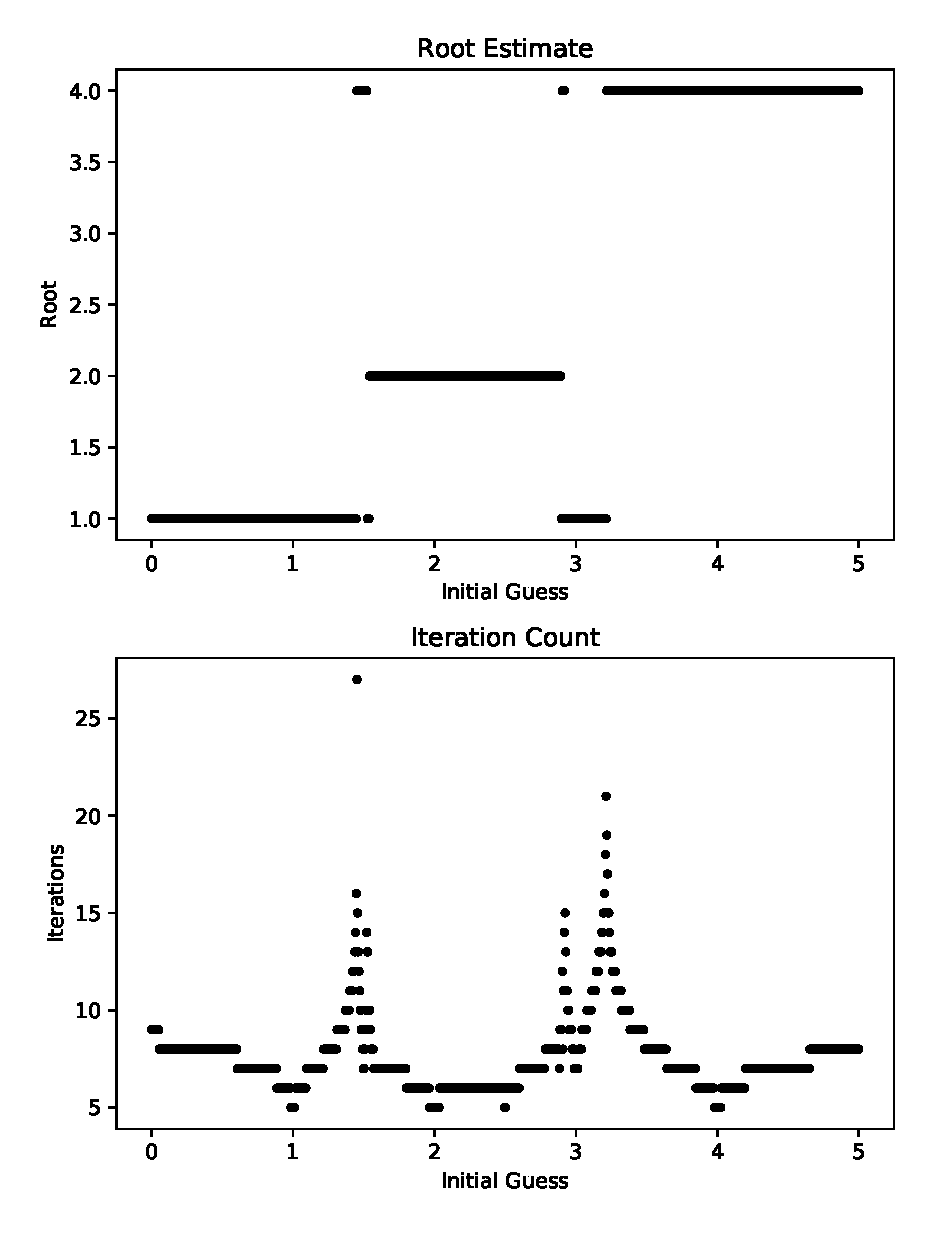
\epsfig{file=RootPlot1.eps} 
\caption{Root Estimates and Iteration Count}
\end{center}
\end{figure}
\begin{figure}[ht!]
\begin{center}
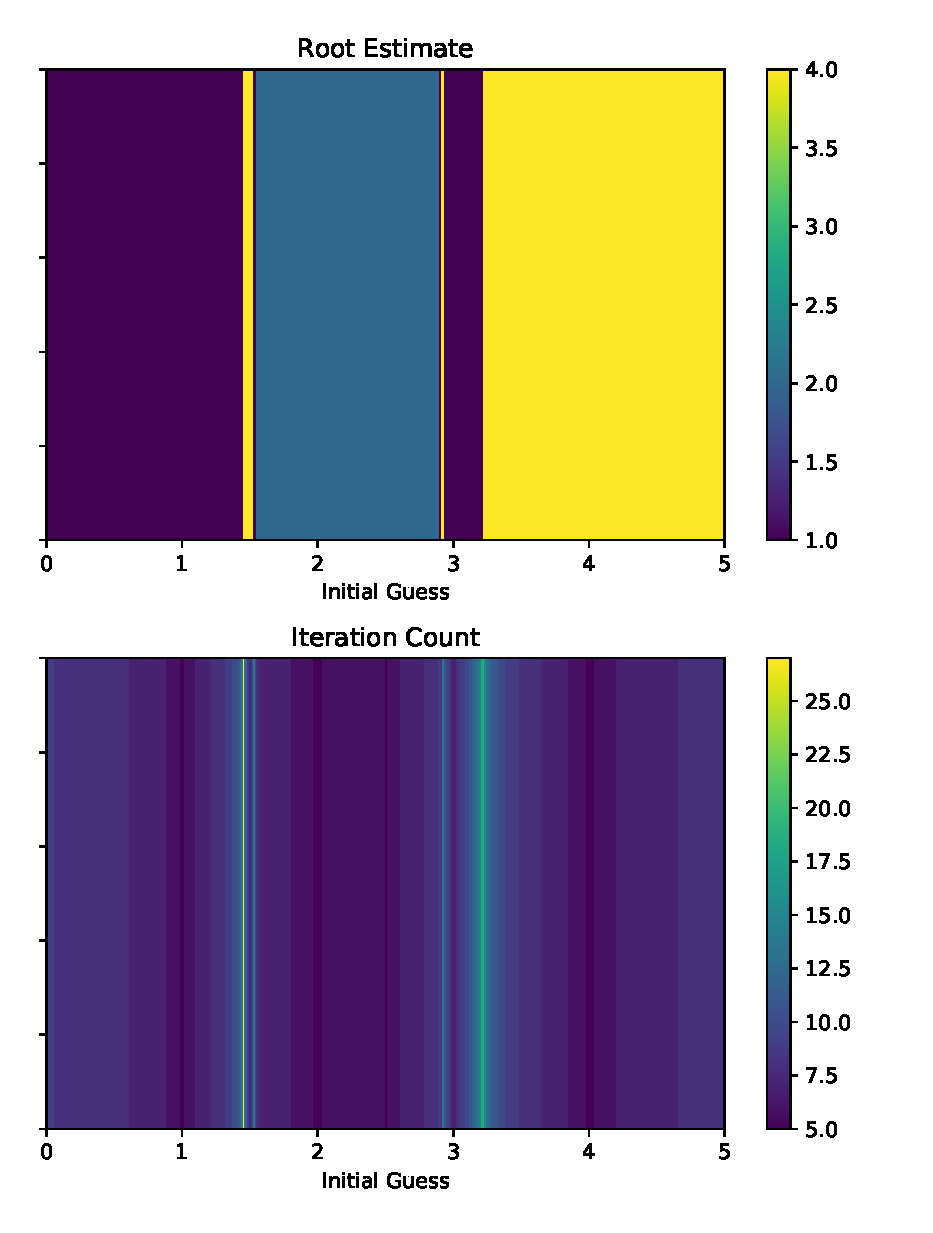
\epsfig{file=RootPlot2.eps} 
\caption{Root Estimates and Iteration Count - As Image}
\end{center}
\end{figure}

\end{document}

